\section{Szeregi formalne i wielomiany wielu zmiennych}

\subsection{Ścisła definicja.}

\begin{definition}
    \begin{enumerate}[label=\arabic*)]
        \item Pierścień szeregów formalnych dwóch zmiennych definiujemy rekurencyjnie jako:
        \[
        R[[X,Y]] := R[[X]][[Y]].
        \]

        \item Dla $n \ge 1$ pierścień szeregów formalnych $n$ zmiennych definiujemy indukcyjnie:
        \[
        R[[X_1,\dots,X_n]] := R[[X_1,\dots,X_{n-1}]][[X_n]].
        \]
        Elementy tego pierścienia utożsamiamy z funkcjami $f \colon \mathbb{N}^n \to R$. 
        Zapisujemy je jako sumy (formalne):
        \[
        \sum_{(i_1,\dots,i_n)\in\mathbb{N}^n} a_{i_1\dots i_n}X_1^{i_1}\cdots X_n^{i_n},
        \]
        gdzie $a_{i_1\dots i_n}=f(i_1,\dots,i_n)$.

        \item Analogicznie, pierścień wielomianów $n$ zmiennych definiujemy indukcyjnie:
        \[
        R[X_1,\dots,X_n] := R[X_1,\dots,X_{n-1}][X_n].
        \]
        Jest to podpierścień pierścienia $R[[X_1,\dots,X_n]]$ złożony z elementów o skończonym nośniku.
    \end{enumerate}
\end{definition}

Pojęcie wielomianu i szeregu formalnego dla jednej zmiennej jest dobrze znane: $X^i$ to ciąg z jedynką na i-tej pozycji. Ale jak to uogólnić na 2, 3, czy n zmiennych? Oto kompletny przewodnik, który krok po kroku pokazuje, jak nasza intuicja rozszerza się wraz ze wzrostem liczby wymiarów.

\subsection{Przypadek n=1: Podstawa, od której wszystko zaczynamy}

\begin{definition}[Pierścień szeregów formalnych jednej zmiennej]
Niech $R$ będzie pierścieniem przemiennym z jedynką. \textbf{Pierścień szeregów formalnych} $R[[X]]$ to zbiór wszystkich nieskończonych ciągów:
\[
(a_0, a_1, a_2, a_3, \dots) \quad \text{gdzie } a_i \in R
\]
z działaniami:
\begin{itemize}
    \item \textbf{Dodawanie:} $(a_0, a_1, \dots) + (b_0, b_1, \dots) = (a_0+b_0, a_1+b_1, \dots)$
    \item \textbf{Mnożenie (splot):} $(a_0, a_1, \dots) \cdot (b_0, b_1, \dots) = (c_0, c_1, \dots)$ gdzie $c_k = \sum_{i+j=k} a_i b_j$
\end{itemize}
\end{definition}

\begin{eg}[Monom $X^i$ dla n=1]
Monom $X^i$ to ciąg z jedynką pierścienia $R$ na i-tej pozycji:
\[
X^0 = (1, 0, 0, 0, \dots) \quad \text{(stała 1)}
\]
\[
X^1 = (0, 1, 0, 0, \dots) \quad \text{(zmienna X)}
\]
\[
X^2 = (0, 0, 1, 0, \dots) \quad \text{(kwadrat X)}
\]
Mnożenie monomów: $X^i \cdot X^j = X^{i+j}$ (splot przenosi jedynkę na pozycję $i+j$).
\end{eg}

\begin{center}
\begin{tikzpicture}
\draw[->] (0,0) -- (6,0) node[right] {indeksy (potęgi X)};
\draw[->] (0,0) -- (0,1.5) node[above] {wartość};
\foreach \x in {0,...,5} {
    \draw (\x,0.1) -- (\x,-0.1) node[below] {$\x$};
}
\filldraw[red] (2,0) circle (2pt) node[above] {1};
\draw[blue, thick] (0,0) -- (1.9,0) (2.1,0) -- (6,0);
\node at (3, -1) {Monom $X^2$: jedynka tylko na pozycji 2};
\end{tikzpicture}
\end{center}

\subsection{Przypadek n=2: Dwie zmienne - dwa sposoby patrzenia}

\subsubsection{Definicja rekurencyjna (pierścień pierścieni)}

\[
R[[X,Y]] := (R[[X]])[[Y]]
\]
Czytamy: bierzemy pierścień szeregów zmiennej $X$, a następnie nad tym pierścieniem budujemy pierścień szeregów zmiennej $Y$.


\begin{eg}[{Element $f \in R[[X,Y]]$}]
Każdy element $f \in R[[X,Y]]$ można zapisać jako szereg względem zmiennej $Y$ o współczynnikach z $R[[X]]$:
\[
f = \sum_{j=0}^\infty f_j Y^j = f_0 + f_1Y + f_2Y^2 + f_3Y^3 + \cdots
\]
gdzie każdy $f_j \in R[[X]]$ jest szeregiem zmiennej $X$:
\[
f_j = \sum_{i=0}^\infty a_{ij} X^i = a_{0j} + a_{1j}X + a_{2j}X^2 + a_{3j}X^3 + \cdots
\]

\textbf{Pełny, rozwinięty zapis:}
\[
f = \underbrace{(a_{00} + a_{10}X + a_{20}X^2 + \cdots)}_{f_0} + \underbrace{(a_{01} + a_{11}X + a_{21}X^2 + \cdots)}_{f_1}Y + \underbrace{(a_{02} + a_{12}X + a_{22}X^2 + \cdots)}_{f_2}Y^2 + \cdots
\]

\textbf{Przykład konkretny:} Niech $f = 1 + 2XY + 3X^2Y^2$. Wtedy:
\begin{align*}
f_0 &= 1 \quad &\text{(szereg stały)} \\
f_1 &= 2X \quad &\text{(szereg liniowy)} \\
f_2 &= 3X^2 \quad &\text{(szereg kwadratowy)} \\
f_j &= 0 \quad &\text{dla } j \geq 3
\end{align*}
Zatem $f = 1 + (2X)Y + (3X^2)Y^2$.
\end{eg}

\subsubsection{Definicja globalna (funkcja na siatce)}

\[
R[[X,Y]] = \left\{ f: \N \times \N \to R \right\}
\]
Element to funkcja, która każdemu punktowi $(i,j)$ na siatce przypisuje współczynnik $a_{ij}$.

\begin{center}
\begin{tikzpicture}[scale=0.8]
\draw[->] (0,0) -- (5,0) node[right] {potęgi X (i)};
\draw[->] (0,0) -- (0,5) node[above] {potęgi Y (j)};
\foreach \x in {0,...,4} {
    \foreach \y in {0,...,4} {
        \draw (\x,\y) circle (2pt);
        \node[below right] at (\x,\y) {$\scriptstyle a_{\x,\y}$};
    }
}
\filldraw[red] (2,3) circle (3pt);
\node[above right] at (2,3) {$(2,3)$};
\node at (2.5, -1) {Każdy punkt siatki ma swój współczynnik};
\end{tikzpicture}
\end{center}

\subsubsection{Monom $X^iY^j$ w obu ujęciach}

\textbf{W ujęciu globalnym:} $X^iY^j$ to funkcja, która przyjmuje wartość 1 w punkcie $(i,j)$ i 0 wszędzie indziej.

\textbf{W ujęciu rekurencyjnym:} $X^iY^j$ to:
\[
X^iY^j = (\underbrace{0, 0, \dots, 0}_{j\text{ zer}}, \underbrace{X^i}_{j\text{-ta pozycja}}, 0, 0, \dots) \in (R[[X]])[[Y]]
\]
Czyli: ciąg względem $Y$, który na j-tej pozycji ma monom $X^i$ (z $R[[X]]$), a na innych pozycjach ma zera.

\subsubsection{Mnożenie dla n=2}

\textbf{W ujęciu globalnym:} Jeśli $f$ ma współczynniki $a_{ij}$, a $g$ ma $b_{ij}$, to $f \cdot g$ ma współczynniki:
\[
c_{ij} = \sum_{\substack{i_1+i_2=i \\ j_1+j_2=j}} a_{i_1j_1} b_{i_2j_2}
\]
To jest \textbf{splot dwuwymiarowy}.

\textbf{Dla monomów:} $X^{i_1}Y^{j_1} \cdot X^{i_2}Y^{j_2} = X^{i_1+i_2}Y^{j_1+j_2}$.

\subsection{Przypadek n=3: Trzy zmienne - hierarchia się pogłębia}

\subsubsection{Definicje}

\textbf{Rekurencyjnie:}
\[
R[[X,Y,Z]] := ((R[[X]])[[Y]])[[Z]]
\]
Interpretacja: najpierw robimy szeregi względem $X$, potem traktujemy je jako współczynniki szeregów względem $Y$, a wynik traktujemy jako współczynniki szeregów względem $Z$.

\textbf{Globalnie:}
\[
R[[X,Y,Z]] = \left\{ f: \N \times \N \times \N \to R \right\}
\]
Element to funkcja, która każdemu punktowi $(i,j,k)$ w \textbf{trójwymiarowej siatce} przypisuje współczynnik $a_{ijk}$.

\subsubsection{Monom $X^iY^jZ^k$}

\begin{center}
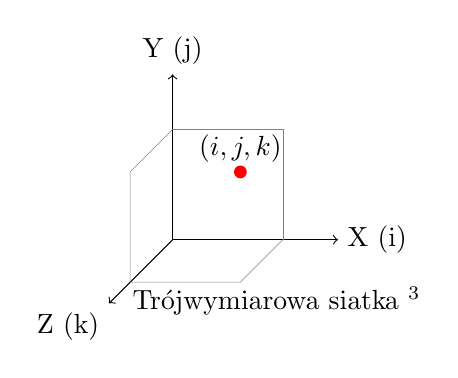
\begin{tikzpicture}[scale=0.7]
\draw[->] (0,0,0) -- (3,0,0) node[right] {X (i)};
\draw[->] (0,0,0) -- (0,3,0) node[above] {Y (j)};
\draw[->] (0,0,0) -- (0,0,3) node[below left] {Z (k)};
\draw[gray, very thin] (2,0,0) -- (2,2,0) -- (0,2,0);
\draw[gray, very thin] (0,2,0) -- (0,2,2) -- (0,0,2);
\draw[gray, very thin] (2,0,0) -- (2,0,2) -- (0,0,2);
\filldraw[red] (2,2,2) circle (3pt);
\node[above] at (2,2,2) {$(i,j,k)$};
\node at (1.5, -1.5, -1) {Trójwymiarowa siatka $\N^3$};
\end{tikzpicture}
\end{center}

\textbf{W ujęciu globalnym:} $X^iY^jZ^k$ to funkcja, która ma wartość 1 w punkcie $(i,j,k)$ i 0 wszędzie indziej.

\textbf{W ujęciu rekurencyjnym:} 
\[
X^iY^jZ^k \in ((R[[X]])[[Y]])[[Z]]
\]
To jest ciąg względem $Z$, który:
\begin{itemize}
\item Na k-tej pozycji ma element $X^iY^j \in (R[[X]])[[Y]]$
\item Na innych pozycjach ma zera $(0,0,\dots)$ z $(R[[X]])[[Y]]$
\end{itemize}
A sam $X^iY^j$ jest z kolei ciągiem względem $Y$, który na j-tej pozycji ma $X^i \in R[[X]]$, a na innych zerami.

\subsubsection{Mnożenie dla n=3}

\textbf{Splot trójwymiarowy:}
\[
c_{ijk} = \sum_{\substack{i_1+i_2=i \\ j_1+j_2=j \\ k_1+k_2=k}} a_{i_1j_1k_1} b_{i_2j_2k_2}
\]

\subsection{Przypadek ogólny: n zmiennych}

\subsubsection{Definicja rekurencyjna}

Dla $n \geq 1$ definiujemy indukcyjnie:
\[
R[[X_1, \dots, X_n]] := (R[[X_1, \dots, X_{n-1}]])[[X_n]]
\]
\textbf{Interpretacja:} Każdy krok dodaje nową "warstwę" rekurencji:
\begin{itemize}
\item Zmienne $X_1, \dots, X_{n-1}$ są "ukryte" w współczynnikach
\item Na najwyższym poziomie pracujemy ze zmienną $X_n$
\end{itemize}

\subsubsection{Definicja globalna}

\[
R[[X_1, \dots, X_n]] = \left\{ f: \N^n \to R \right\}
\]
gdzie $\N^n = \underbrace{\N \times \N \times \cdots \times \N}_{n \text{ razy}}$.

\textbf{Interpretacja:} Każdy element to funkcja na n-wymiarowej siatce. Punkt $(i_1, i_2, \dots, i_n)$ na tej siatce odpowiada monomowi $X_1^{i_1}X_2^{i_2}\cdots X_n^{i_n}$.

\subsubsection{Monom $X_1^{i_1}\cdots X_n^{i_n}$}

\textbf{W ujęciu globalnym:} To funkcja $f: \N^n \to R$ taka, że:
\[
f(j_1, \dots, j_n) = 
\begin{cases}
1 & \text{jeśli } (j_1, \dots, j_n) = (i_1, \dots, i_n) \\
0 & \text{w przeciwnym przypadku}
\end{cases}
\]

\textbf{W ujęciu rekurencyjnym:} To element z $(R[[X_1, \dots, X_{n-1}]])[[X_n]]$:
\[
X_1^{i_1}\cdots X_n^{i_n} = (0, \dots, 0, \underbrace{X_1^{i_1}\cdots X_{n-1}^{i_{n-1}}}_{i_n\text{-ta pozycja}}, 0, \dots)
\]
A sam $X_1^{i_1}\cdots X_{n-1}^{i_{n-1}}$ definiujemy rekurencyjnie analogicznie.

\subsubsection{Mnożenie w n wymiarach}

Jeśli $f$ ma współczynniki $a_{i_1\dots i_n}$, a $g$ ma $b_{i_1\dots i_n}$, to ich iloczyn $h = f \cdot g$ ma współczynniki:
\[
c_{i_1\dots i_n} = \sum_{\substack{j_1+k_1 = i_1 \\ \vdots \\ j_n+k_n = i_n}} a_{j_1\dots j_n} b_{k_1\dots k_n}
\]
To jest \textbf{splot n-wymiarowy}.

\subsection{Tabela porównawcza: od n=1 do n ogólnego}

\begin{center}
\begin{tabular}{|c|c|c|c|}
\hline
\textbf{n} & \textbf{Przestrzeń} & \textbf{Monom} & \textbf{Splot (mnożenie)} \\
\hline
1 & $\N$ & $X^i$ = 1 na $i$ & $c_k = \sum_{i+j=k} a_i b_j$ \\
\hline
2 & $\N \times \N$ & $X^iY^j$ = 1 na $(i,j)$ & $c_{ij} = \sum_{\substack{i_1+i_2=i \\ j_1+j_2=j}} a_{i_1j_1} b_{i_2j_2}$ \\
\hline
3 & $\N \times \N \times \N$ & $X^iY^jZ^k$ = 1 na $(i,j,k)$ & $c_{ijk} = \sum_{\substack{i_1+i_2=i \\ j_1+j_2=j \\ k_1+k_2=k}} a_{i_1j_1k_1} b_{i_2j_2k_2}$ \\
\hline
n & $\N^n$ & $X_1^{i_1}\cdots X_n^{i_n}$ = 1 na $(i_1,\dots,i_n)$ & $c_{i_1\dots i_n} = \sum_{\substack{j_1+k_1=i_1 \\ \vdots \\ j_n+k_n=i_n}} a_{j_1\dots j_n} b_{k_1\dots k_n}$ \\
\hline
\end{tabular}
\end{center}

\subsection{Równoważność obu podejść - kluczowe twierdzenie}

\begin{theorem}[Równoważność definicji]
Dla dowolnego $n \geq 1$ i dowolnego pierścienia przemiennego $R$ z jedynką, istnieje naturalny izomorfizm pierścieni:
\[
(R[[X_1, \dots, X_{n-1}]])[[X_n]] \cong \left\{ f: \N^n \to R \right\}
\]
który utożsamia monom $X_1^{i_1}\cdots X_n^{i_n}$ z funkcją mającą 1 w punkcie $(i_1,\dots,i_n)$.
\end{theorem}

\subsubsection*{Jak działa ten izomorfizm?}

Z lewej do prawej: weźmy element $F \in (R[[X_1,\dots,X_{n-1}]])[[X_n]]$. Zapiszmy go jako:
\[
F = \sum_{k=0}^\infty F_k X_n^k \quad \text{gdzie } F_k \in R[[X_1,\dots,X_{n-1}]]
\]
Każdy $F_k$ to funkcja $\N^{n-1} \to R$. Wtedy odpowiadająca funkcja $f: \N^n \to R$ to:
\[
f(i_1,\dots,i_{n-1}, i_n) = F_{i_n}(i_1,\dots,i_{n-1})
\]

\subsection{Praktyczne wskazówki: Kiedy używać którego podejścia?}

\begin{itemize}
\item \textbf{Użyj podejścia rekurencyjnego} gdy:
  \begin{itemize}
  \item Dowodzisz twierdzenia przez indukcję względem liczby zmiennych
  \item Pracujesz z algorytmami rekurencyjnymi
  \item Chcesz "ukryć" złożoność do czasu, aż będzie potrzebna
  \end{itemize}

\item \textbf{Użyj podejścia globalnego} gdy:
  \begin{itemize}
  \item Badasz symetrie między zmiennymi
  \item Pracujesz ze stopniem całkowitym
  \item Robisz obliczenia kombinatoryczne
  \item Wizualizujesz problem geometrycznie
  \end{itemize}
\end{itemize}

\subsection*{Podsumowanie: Od linii do n-wymiarowej przestrzeni}

\begin{itemize}
\item \textbf{n=1:} To linia. Każdy punkt to potęga jednej zmiennej.
\item \textbf{n=2:} To płaszczyzna. Każdy punkt to para potęg (dwóch zmiennych).
\item \textbf{n=3:} To przestrzeń 3D. Każdy punkt to trójka potęg.
\item \textbf{n ogólne:} To n-wymiarowa przestrzeń. Każdy punkt to n-tka potęg.
\end{itemize}

\noindent
\textbf{Kluczowa idea:} Niezależnie od liczby wymiarów, monom to zawsze "jedynka w jednym punkcie przestrzeni, zera wszędzie indziej". Mnożenie to przesuwanie i sumowanie tych jedynek zgodnie z zasadą dodawania wykładników.


